\chapter{Astrophysics around neutron stars}
\chapterimage[width=15cm]{wordcloud/chap3b.png}

Let us next discuss the violent environments of neutron stars and the related astrophysics therein.
These surroundings also play an important role when we try to decipher different kinds of observations of neutron stars.
In the heart of this whole problem is an astrophysical process called accretion.
This is a process where matter is transferred from one source to another because of the gravitational forces.
Most importantly, the infalling material has to somehow lose its angular momentum before it is able to travel all the way to the neutron star surface.
Nature's platform for this is called an accretion disk.
Sometimes the disk also continues all the way to the surface of the neutron star.
Instead of smoothly joining the star, this process is often violent and leads to another source of radiation as this so-called boundary layer heats up when the rapidly rotating inner disk tries to slow down to velocities similar to that of the more gently rotating star.

We begin by discussing the basics of the accretion process and present some order-of-magnitude estimates relevant for the accretion disks and boundary layers.
Most importantly, we try to characterize the strength of the radiation originating from them.
Lastly, we will also discuss the unstable thermonuclear runaways, X-ray bursts, that can be seen as the end-results of this accretion.


\section{Accretion}

Accretion is an astrophysical process that has its roots in the gravitational potential energy.
It can be a source of an enormous amount of energy if the central object is compact, because the depth of a gravitational well is directly proportional to the compactness of the central source.
Hence, it is an important, and often dominating, process for neutron stars.\cite[see e.g.,][]{FKR02}

Gravitational potential energy release for a mass $m$ that is accreted onto a compact object of radius $R$ and mass $M$ is
\be
\Delta E_{\mathrm{acc}} = m \frac{G M}{R} \sim 10^{20} \left( \frac{m}{\g} \right) \left( \frac{10\km}{R} \right) \left( \frac{M}{\Msun} \right) \erg,
\ee
where in the latter expression typical dimensions of neutron star are used.

This energy, $10^{20} \erg$ per each gram that is accreted, is usually released as radiation.
The rate of this energy release is simply related to the mass accreted per unit time, i.e., accretion rate $\Mdot = \Delta M/ \Delta t$, 
\be
L_{\mathrm{acc}} = \Mdot \frac{G M}{R} \approx \Ten{1.3}{36} \left( \frac{\Mdot}{10^{16} \g\unitspace\mathrm{s}^{-1}} \right) \left( \frac{10\km}{R} \right) \left( \frac{M}{\Msun} \right) \ergs,
\ee
where a typical value of $\Mdot \sim 10^{16} \g\unitspace\mathrm{s}^{-1} \approx \Ten{1.5}{-10} \Msun\unitspace\mathrm{yr}^{-1}$ is taken for the accretion rate.
For higher accretion rate, $L_{\mathrm{acc}}$ can reach the Eddington luminosity (Eq. \eqref{eq:Ledd}) of a neutron star.

%\red{X-rays from blackbody $T$}


\subsection{Roche lobes and mass transfer in binary systems}

In order to use the accretion as an energy source, mass transfer needs to take place in the system.
For the mass transfer to keep on operating, a source of fresh material is needed.
In binary systems with two stars, the companions star is the obvious fuel resource.
Here we will focus on the so-called Low Mass X-ray Binary (LMXB) systems where the companion, like the name implies, is a relatively low-mass star with a mass $M \lesssim 1 \Msun$.\cite{TH06}
%Typically, it is a normal or a late-type star with a mass $M \lesssim 1 \Msun$.
Such a setup leads to a mass-transfer quite naturally as the heavier neutron star will just rip out the outer layers of its poor companion and slowly devours it, until nothing is left.
As another option, the system could be a so-called High Mass X-ray Binary (HMXB) system, where the companion of the neutron star has $M \sim 10\Msun$, and the accretion happens, for example, via a neutron star capturing the strong wind from the companion.
Here in this thesis, we will, however, only focus on the LMXB systems.


%Roche Lobe \cite{PRP02} \cite{LL15}
How exactly is the material transferred from the companion to the primary star is an interesting problem.
We can begin to understand the physical setup by considering a general hydrodynamical system of two objects in a rotating frame.
Here we select the frame that co-rotates with the binary system. % with an angular velocity $\omega$.
The subsequent flow of gas between the two stars can then be described by the Euler equation with additional Coriolis and centrifugal terms.\cite[see e.g.,][]{Cho98}
In practice the Euler equation describes the time evolution of the velocity $\vec{v}$ of the gas that has a pressure $P$ and density $\rho$.
In a reference frame rotating together with the binary system with angular velocity $\omega$ the Euler equation takes the form 
\be
\frac{ \partial \vec{v} }{\partial t} + (\vec{v} \cdot \nabla)\vec{v} = -\nabla \Phi_{\mathrm{R}} - 2 \vec{ \omega } \times \vec{v} - \frac{1}{\rho} \nabla P,
\ee
where the angular velocity of the binary is
\be
\vec{ \omega } = \left( \frac{ G M }{a^3} \right)^{1/2} \vec{e},
\ee
as given with the unit vector $\vec{e}$ normal to the orbital plane.
Here $M$ is the total mass of the system, i.e., $M = M_1 + M_2$, where $M_1$ and $M_2$ are the individual masses of the two stars in the system, respectively, and $a$ is their orbital separation.

\begin{figure}[t!]
%\centering
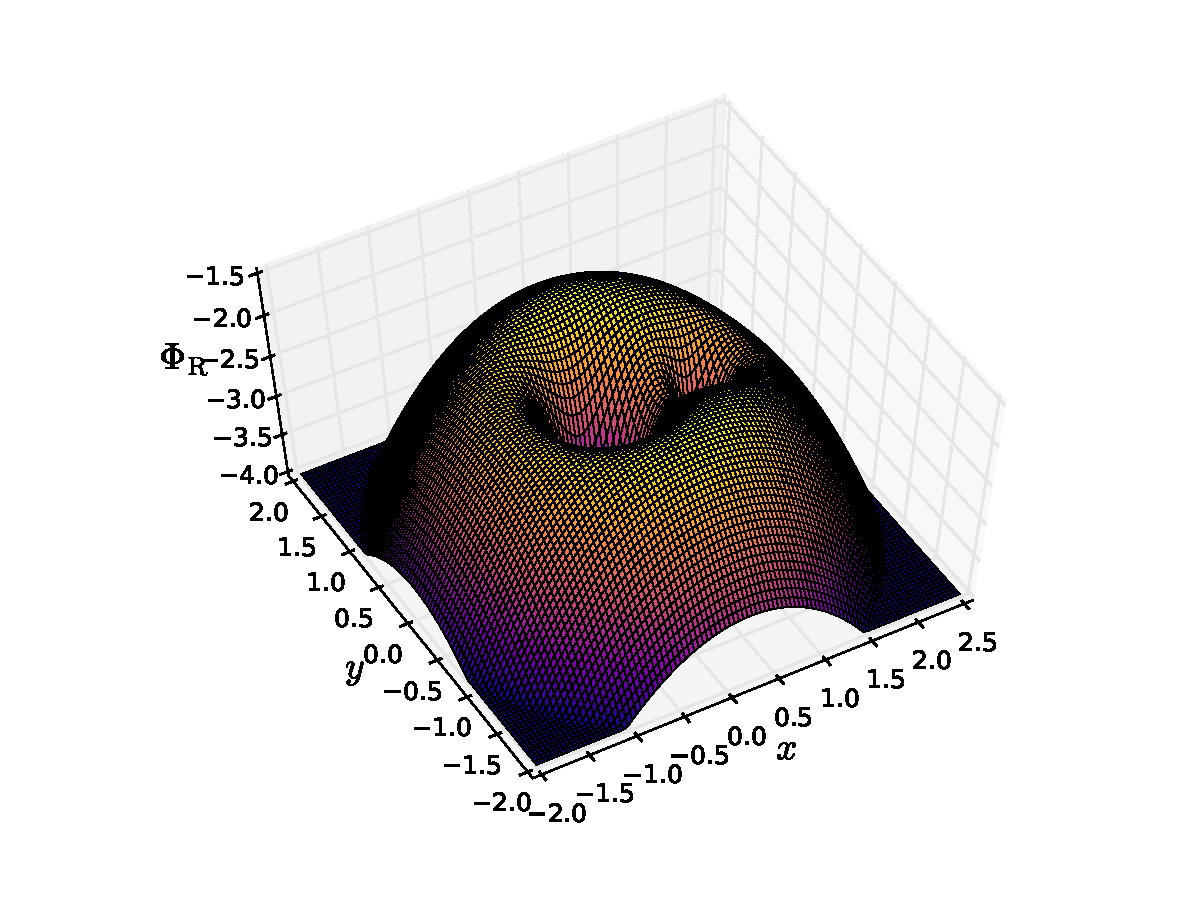
\includegraphics[width=16cm]{figs/astro/roche.pdf}
\caption{\label{fig:roche}
    Two-dimensional Roche potential $\Phi_{\mathrm{R}}(x,y)$ visualized for a binary systems with $M_1/M_2 = 0.25$ and $a = 1$. 
    The nozzle ($L_1$ point) is visible as a valley (or more specifically, a saddle point) between the gravitational wells of the two stars.
}
\end{figure}

The effects originating from the gravitation and from the centrifugal forces are encapsulated in the so-called Roche potential, given as a function of radial vector $\vec{r}$ as\cite[see e.g.,][]{PRP02, LL15}
\be
\Phi_{\mathrm{R}}(\vec{r}) = -\frac{G M_1}{|\vec{r} - \vec{r_1}|} -\frac{G M_2}{|\vec{r} - \vec{r_2}|} - \frac{1}{2} ( \vec{ \omega } \times \vec{r} )^2,
\ee
where the location of the stars are given with $\vec{r_1}$ and $\vec{r_2}$.
By studying the shape of the potential, we see that in between the two stars, in the so-called $L_1$ point there exists a location where the countering gravitational forces from the two stars are balanced.
This can be thought of as a physical nozzle in the system from which the less massive star will leak material into the more massive star.
Such a mass transfer, also known as a Roche lobe overflow, will then occur if the companion star's radius exceeds the size of its own individual Roche lobe visualized in \fig{fig:roche}.
Typically such a thing can happen when the star evolves and expands at the end of its life cycle. 


\subsection{Accretion disks}
%accretion disk: machine for slowly lowering material in the graviational potential and extracting energy.
%orbital kinetic energy to heat

When the mass transfer has started via the Roche lobe overflow, and we have a stable source of material that is being transferred from the companion to the more massive neutron star, we can next focus on the region where gravitational forces of the neutron star dominate.
Originally, we can think of each individual incoming particle having their own circular orbit around the central object.
The mass flow, i.e., the stream of particles, is confined into the orbital plane of the binary system, hence, the problem of describing the physics of the flow is one dimensional as a first approximation because only radial coordinate $r$ is considered.
This is known as the so-called thin-disk approximation.
The nested circular orbits of the plasma can be naturally described in cylindrical coordinates, hence the word ``disk''.
Secondly, the scale height $H$ of the disk is small compared to the radial coordinate ($H \ll r$), so we say that the disk is thin.

Radial structure of the disk can then be obtained from the Keplerian rotation law as
\be
\Omega_{\mathrm{K}}(r) = \left( \frac{G M }{r^3} \right)^{1/2},
\ee
describing an angular velocity as a function of radial coordinate from the disk center.
There is an important detail hidden here in the Kepler's law:
Keplerian angular velocity implies differential rotation, i.e., varying angular velocities as a function of $r$.
Such a shearing between two adjacent annuli will then lead to viscous stresses. % when the inner annulus rotates faster than the outer one.

The disk's structure can be obtained from the hydrodynamical equations in cylindrical coordinates.
Instead of the density $\rho$, let us use the surface density $\Sigma = 2 H \rho$ to describe the mass. %&, where $H$ is the scale height of the disk.
Conservation of mass and angular momentum can then be written as\cite[see e.g.,][]{Cho98, FKR02}
\be\label{eq:disk_1}
r \frac{\partial \Sigma}{\partial t} + \frac{\partial}{\partial r}(r \Sigma v_r) = 0,
\ee
and
\be\label{eq:disk_2}
r \frac{\partial}{\partial t}(\Sigma r^2 \Omega) + \frac{\partial}{\partial r} (r \Sigma v_r r^2 \Omega) = \frac{1}{2\pi} \frac{\partial \tau}{\partial r},
\ee
where $v_r$ is the velocity in $r$ direction and $\tau$ is the viscous torque of the differentially rotating disk.

Torque, in general, can be understood as an angular momentum flux density per unit time and is given by
\be
\tau_i = \epsilon_{ijk} r_j f_k,
\ee
where $\epsilon_{ijk}$ is the Levi-Civita symbol, and $f_k$ is the force density, i.e., momentum density flux per unit time, given as
\be
f_k = \sigma_{kh} n_h.
\ee
Here $\sigma_{kh}$ is the $kh$-component of a general stress tensor $\sigma_{ij}$, and $n_h$ is some surface normal of the area where the shearing takes place.
In our case, we can compute the shear in cylindrical coordinate system focusing on $r$ and $\phi$ coordinates only as\cite[see e.g.,][]{Cho98}
\be
\sigma_{r\phi} = \rho \nu \left( r \frac{\partial}{dr} \left\{\frac{v_{\phi}}{r}\right\} + \frac{1}{r} \frac{d v_r}{d\phi} \right),
\ee
which simplifies to 
\be
\sigma_{r\phi} = \rho \nu r \frac{d\Omega}{d r},
\ee
when we remember that $v_{\phi} = r \Omega$ and assume the flow to be symmetric in the azimuthal $\phi$-direction ($\partial v_r/\partial \phi = 0)$.
The total viscous torque acting at the $2\pi r (2 H)$ area corresponding to the disk rim at location $r$ is then
\be
\tau(r,t) = 2\pi r \nu \Sigma r^2 \frac{d \Omega}{d r}.
\ee
%where $\Omega' = d\Omega/dr$.

Combining the latter expressions and assuming Keplerian rotation $\Omega(r) = \Omega_{\mathrm{K}}(r)$ with a fixed central mass of $M$ (i.e., $\partial\Omega/\partial t = 0$), we can then solve the system of equations and obtain expressions for the surface density and the radial velocity as
\be\label{eq:disk_st_1}
\frac{\partial \Sigma}{\partial t} = \frac{3}{r} \frac{\partial}{\partial r} \left[ r^{1/2} \frac{\partial}{\partial r} (\nu \Sigma r^{1/2}) \right],
\ee
and
\be\label{eq:disk_st_2}
v_r = -\frac{3}{\Sigma r^{1/2}} \frac{\partial}{\partial r} ( \nu \Sigma r^{1/2}).
\ee
In order to continue further, we would need a description for the viscosity $\nu$.
It could have its roots on the normal molecular viscosity\cite{ChapmanCowling52} or like the current theories imply, be magnetohydrodynamic in nature.
The latter is known as the magnetorotational instability (MRI) where magnetic stresses of turbulent field lines cause viscosity for the plasma. \cite{Velikhov59, Cha60, BH91} 
As another approach, we should also mention the widely successful $\alpha$ parameterization by Shakura \& Sunyaev, known as the ``standard disk'' or $\alpha$-disk.\cite{SS73}
This method is mostly mathematical as we just reparameterize our ignorance of the viscosity into a new parameter called $\alpha$, that is taken to be proportional to the local soundspeed $c_{\mathrm{s}}$ and height of the disk $H$, as $\nu = \alpha c_{\mathrm{s}} H$.
Even though only mathematical in nature, this formulation has turned out to be extremely successful in helping to explain the basic functionality of accretion disks because $\alpha$ can be treated as a small parameter in all the subsequent formulae.
The physical reason for the smallness of $\alpha$ is also intuitive: velocities can not be larger than the local soundspeed, otherwise supersonic flows would produce shocks that would dissipate energy until the local velocities are subsonic again.
Similarly, the size of the turbulent eddies must be smaller than the disk scale height. 
Together these then imply $\alpha \lesssim 1$.

To get some idea of the disk dynamics, we can, as our zeroth order approximation assume $\nu = \mathrm{constant}$.
Then, the time-dependent disk structure (Eqs. \eqref{eq:disk_1} and \eqref{eq:disk_2}) can be solved, for example, by assuming as an initial condition a ring of mass $m$ at $r=r_0$,
\be
\Sigma(r,t=0) = \frac{m}{2\pi r_0} \delta(r - r_0),
\ee
where $\delta$ is the Dirac delta function.
As a solution, we then obtain a mass distribution that slowly diffuses due to viscosity as
\be\label{eq:sigma}
\Sigma(\tilde{r},\tilde{t}) = \frac{m}{\pi r^2} \frac{1}{\tilde{t} ~ \tilde{r}^{1/4} } \exp\left[-\frac{(1+\tilde{r}^2)}{\tilde{t}}\right] I_{1/4}\left(\frac{2\tilde{r}}{\tilde{t}}\right),
\ee
where $I_{1/4}(x)$ is the modified Bessel function, $\tilde{r} \equiv r/r_0$ is the dimensionless radial coordinate, and $\tilde{t} \equiv 12 \nu t /r_0^2$ is the dimensionless time.
Inserting \eqref{eq:sigma} into \eqref{eq:disk_st_2}, we also obtain
\be
v_r(\tilde{r}, \tilde{t}) = -\frac{3 \nu}{r_0} \frac{\partial}{\partial \tilde{r}} \left[ \frac{1}{4} \ln \tilde{r} - \frac{(1+\tilde{r}^2)}{\tilde{t}} + \ln I_{1/4}\left(\frac{2\tilde{r}}{\tilde{t}} \right) \right].
\ee
Which in the asymptotic limits give
\be
v_r \sim 
\begin{cases}
  \phantom{+}\displaystyle\frac{3\nu}{r_0} \left(\frac{1}{4\tilde{r}} + \frac{2\tilde{r}}{\tilde{t}} - \frac{2}{\tilde{t}} \right) > 0 \quad & \text{for } 2\tilde{r} \gg \tilde{t} \\
    -\displaystyle\frac{3\nu}{r_0} \left(\frac{1}{2\tilde{r}} - \frac{2\tilde{r}}{\tilde{t}} \right) < 0 \quad & \text{for } 2\tilde{r} \ll \tilde{t}. \\
\end{cases}
\ee
Even from this simplified treatment we can understand the basic physics of how the accretion disks operate:
The viscous shear stresses help the rotating plasma redistribute its angular momentum outwards while at the same time most of the mass is accreted inwards.


Let us next study a steady-state disk solution by setting $\partial/\partial t \rightarrow 0$.
From the angular momentum conservation \eqref{eq:disk_2} we obtain
\be\label{eq:ssdisk}
r \Sigma v_{r} r^2 \Omega = \frac{\tau}{2\pi} + \frac{C}{2\pi},
\ee
with a constant $C$ that physically represent a torque term from the coupling of the inner disk and the star at $r \approx R$.
In short,%
\footnote{Torque is alternatively defined via the linear momentum $\vec{p} = m v_{\phi} \vec{\hat{e}_{\phi}}$, as $\tau = d(\vec{r} \times \vec{p})/dt = r v_{\phi} dm/dt = r^2 \Omega \Mdot$. 
This represents again the flow of angular momentum in the system.
}
it is given by
\be\label{eq:visc_torque}
C \approx -\Mdot(R) R^2 \Omega(R) \approx -\Mdot R^2 \Omega_{\mathrm{K}}(R) = -\Mdot (G M R)^{1/2},
\ee
with the expression for the mass accretion rate given in terms of the radial velocity $v_r$ as
\be
\Mdot(r) = -\frac{2\pi r \Sigma dr}{dt} = -2\pi r \Sigma v_r,
\ee
and assuming a thin layer for the zone where the inner disk angular velocity is slowed down to the angular velocity of the star (otherwise we could not set $r \rightarrow R$).
Substituting this into \eqref{eq:ssdisk}, and assuming Keplerian angular velocity profile, we obtain
\be
\nu \Sigma = \frac{\Mdot}{3\pi} \left[ 1 - \left( \frac{R}{r}\right)^{1/2}  \right].
\ee
Physically this represents a steady-state solution of a disk with central torque applied to it.
Viscous dissipation rate per unit disk face area is then%
\footnote{Viscous dissipation rate in ring of width $dr$ is $\tau \Omega' dr$, i.e., the rate of work done by the torque, and the total area of the ring, taking into account both the lower and upper faces, is $4\pi r dr$. Hence, we obtain Eq. \eqref{eq:D} as the ratio of these.
}
\be\label{eq:D}
D(r) = \frac{\tau \Omega'}{4\pi r} = \frac{1}{2} \nu \Sigma (r \Omega')^2 = \frac{3 G M \Mdot}{8 \pi r^3} \left[ 1 - \left( \frac{R}{r}\right)^{1/2}  \right].
\ee
Finally, from here we can compute the luminosity of the disk faces due to energy lost by viscous dissipation
\begin{align}\begin{split}
    L(r_1, r_2)  &= 2 \int_{r_1}^{r_2} D(r) 2\pi r dr = \frac{3 G M \Mdot}{2} \int_{r_1}^{r_2} \left[ 1 - \left( \frac{R}{r} \right)^{1/2} \right] \frac{dr}{r^2} \\
 & = \frac{3 G M \Mdot}{2} \left\{ \frac{1}{r_1} \left[ 1 - \frac{2}{3}\left( \frac{R}{r_1} \right)^{1/2} \right] -  \frac{1}{r_2} \left[ 1 - \frac{2}{3}\left( \frac{R}{r_2} \right)^{1/2} \right] \right\}, 
\end{split}\end{align}
and by then setting $r_1 \rightarrow R$ and $r_2 \rightarrow \infty$, we get
\be
L_{\mathrm{disk}} = \frac{G M \Mdot}{2 R} = \frac{1}{2} L_{\mathrm{acc}}.
\ee
Hence, half of the potential energy will be lost by the viscous shearing and is radiated away by the upper and lower faces of the accretion disk.
Importantly, the other remaining half will be transferred all the way to the star.

Temperature of the hottest inner disk can be estimated by assuming an optically thick media and using the dissipation rate $D$ as the surface flux.
This innermost region of the disk is the brightest as here the gravity is the strongest and the dissipation area the smallest.
Estimate for the disk surface temperature can then be obtained from
\be
\sigma_{\mathrm{SB}} T_{\mathrm{disk}}^4(r) \sim D(r).
\ee
From here we obtain
\be
T_{\mathrm{disk}}(r) = T_{*} \left[ 1- \left( \frac{R}{r} \right)^{1/2} \right]^{1/4} \left(\frac{R}{r}\right)^{3/4},
\ee
where
\be
T_{*} = \left( \frac{3 G M \Mdot}{8 \pi R^3 \sigma_{\mathrm{SB}}} \right)^{1/4} 
\approx \Ten{2.3}{7} \left(\frac{\Mdot}{10^{16} \g\unitspace\mathrm{s}^{-1}}\right)^{1/4} \left(\frac{M}{\Msun}\right)^{1/4} \left(\frac{R}{10\km}\right)^{-3/4} \Kelvin,
\ee
is a typical temperature in the innermost regions of the disk.


%Reynolds number for the disk (inertia / viscous dissipation)
%\be
%\mathcal{R} \sim \frac{ v_{\phi}^2 / R }{\lambda \bar{v} v_{\phi} /R^2} = \frac{R v_{\phi}}{\lambda \bar{v}}
%\ee
%Molecular viscosity for $\lambda \sim \lambda_{\mathrm{D}}$ and $\bar{v} \sim c_{\mathrm{s}}$.
%For typical accretion disk environment molecular $\mathcal{R} > 10^{14}$, i.e. highly turbulent.
%Typical size of the turbulent eddies can not exceed the disk thickness $H$.
%Velocity is most likely below sound speed $c_{\mathrm{s}}$ as otherwise turbulent motions would be thermalized by shocks from the supersonic motion.
%Hence
%\be
%\nu = \alpha c_{\mathrm{s}} H
%\ee
%and we expect $\alpha \lesssim 1$. 
%Reparameterizaton of our ignorance.
%This is the $\alpha$-prescription by Shakura and Sunyaev.\cite{SS73}
%
%\cite{Cho98}
%Hydrodynamics of disks.

\begin{figure}[t!]
\centering
\includegraphics[width=12cm]{figs/astro/fig_disk_soft.png}
\includegraphics[width=12cm]{figs/astro/fig_disk_hard.png}
\caption{\label{fig:disk}
    Schematic view of the two different accretion states.
    \emph{Top:} Soft state with inner disk extending all the way down to the neutron star surface.
    \emph{Bottom:} Hard state with truncated disk and hot inner flow (red).
}
\end{figure}

Observationally we see that the disks are, however, not as simple as discussed here.\cite[see e.g.,][for a review]{DGK07}
The standard $\alpha$-disk model assumes steady-state, whereas in reality the disk structure evolves in time.
Most importantly, the mass accretion rate is seen to vary over long timescales.
From observations we also know that the disks alternates between two states called hard and soft state.\cite{Mitsuda89, HvdK89, GD02, MC03, MDF14, DGK07}

The soft (also known as ``high'' or ``thermal-dominant'') state is characterized by a strong soft component in the observed spectra.\cite[see e.g.,][]{GZP99}
There is, however, also a complex non-thermal tail usually present.\cite{MRC00}
Here the soft component could be interpreted as a thermal radiation from an optically thick disk but the non-thermal tail implies that this picture is not complete.
The hard (also known as ``low'') state is even more complicated as the observational spectra is dominated by a strong hard X-ray component but some signs of a low-temperature thermal disk is also sometimes visible.\cite{ZG04}

The current physical interpretation of these two states can be satisfactorily explained by a truncated disk model with a hot inner flow.
Here the disk, well-described by the Shakura \& Sunyaev $\alpha$-disk is truncated, i.e., does not always reach the central object.
The cool and optically thick, geometrically thin, disk is then responsible of the low-energy thermal radiation.
In the innermost parts, the disk turns into hot, optically thin flow, that is also responsible for the non-thermal radiation component.
Depending on the mass accretion rate, the disk truncation radius varies and so the strength of the thermal disk and hot inner flow components can vary.
To simplify, this means that hard state typically corresponds to a low accretion rate and soft state to a high mass accretion rate.


\subsection{Boundary layers}

Our simple analysis of accretion disk physics has shown that viscous dissipation can get rid of up to half of the potential energy of the incoming matter.
Where the other half goes, we shall look next.

Imagine the accretion disk extending all the way down to the central star.
The angular frequency of this disk edge can be taken to be Keplerian, $\Omega_{\mathrm{K}}(R)/2\pi \sim 1500 \unitspace\mathrm{Hz}$.
The star, on the other hand, usually rotates anywhere from $100$ to $600$ revolutions per second.\cite{Watts12, PTR14}
Hence, we expect a thin interface between the star and the disk where angular velocity changes by a factor of $\sim 3$ to $15$.
This region we call the boundary layer.

Let us assume a thin layer of width $b$ so that $\Omega(R + b) \approx \Omega_{\mathrm{K}}(R + b)$. % corresponding to the disk rim just before this layer.
Within this layer, the angular velocity should decrease to $\Omega_*$ as we move from radial location $R+b$ to $R$ towards the star's surface.
The viscous torque to spin up the star is then, similar to \eqref{eq:visc_torque}, written as
\be
\tau_* = \Mdot R^2 (\Omega_{\mathrm{K}} - \Omega_*).
\ee
Rate of the kinetic energy change, on the other hand, is simply obtained by considering the difference of the kinetic energies per time as
\be
\dot{E} = \frac{1}{2} \Mdot R^2 (\Omega_{\mathrm{K}}^2 - \Omega_{*}^2) = 
\frac{1}{2} \Mdot \frac{GM}{R} \left[ 1 - \left(\frac{\Omega_*}{\Omega_{\mathrm{K}}} \right)^2 \right] 
\ee
For the expression of the total rate of energy change we need to subtract the work done by the viscous torque per unit time, $\tau \Omega_*$, to get %TODO
\be
L_{\mathrm{BL}} = \frac{1}{2} \Mdot R^2 (\Omega_{\mathrm{K}}^2 - \Omega_{*}^2) - \Mdot R^2 \Omega_* (\Omega_{\mathrm{K}} - \Omega_* )
 = \frac{1}{2} \frac{G M \Mdot}{R} \left( 1 - \frac{\Omega_*}{\Omega_{\mathrm{K}}} \right)^2
\ee
In the limit $\Omega_* \ll \Omega_{\mathrm{K}}$ we obtain
\be
L_{\mathrm{BL}} = \frac{1}{2}  \frac{G M \Mdot}{R} = \frac{1}{2} L_{\mathrm{acc}}.
\ee

Let us finally estimate the temperature of this layer.
By assuming an optically thick emitting region, we get a characteristic blackbody temperature again from
\be\label{eq:BLT}
A_{\mathrm{BL}} \sigma_{\mathrm{SB}} T_{\mathrm{BL}}^4 \sim L_{\mathrm{BL}},
\ee
where $A_{\mathrm{BL}}$ is the area of the emitting region.
As a reasonable first guess we can use $b \sim H$ so an annulus around the star has an area of $A_{\mathrm{BL}} = 2\times2\pi R H$ taking into account both top and bottom face.
This corresponds to a temperature of
\be
T_{\mathrm{BL}} \sim \left( \frac{G M \Mdot}{8\pi \sigma_{\mathrm{SB}} R^2 H} \right)^{1/4} \sim T_{*} \left( \frac{R}{H} \right)^{1/4}
\ee

As another option we can consider a so-called spreading layer.\cite{IS99, SP06}
Instead of assuming that the energy is dissipated in a thin equatorial ring, we can assume that it will spread to cover the whole star.
In this case, $A_{\mathrm{SL}} \sim 4\pi R^2$, and using Eq. \eq{eq:BLT}, we get 
\be
T_{\mathrm{SL}} \sim T_{*},
\ee
i.e., a smaller temperature ($T_{\mathrm{SL}} < T_{\mathrm{BL}}$) that is comparable to the temperature of the disk.

Finally, one should note that the physical processes discussed here assume Newtonian gravity.
In a general relativistic treatment the energy release in the boundary layer can be almost two times that of the energy released in the disk.\cite{SS86, SS00}



\section{X-ray bursts and unstable thermonuclear burning}\label{sect:bursts}

Accretion can be a powerful energy source but this is not he end of the material that slowly spirals down into the star.
After it has traveled all the way to the surface of the neutron star, it will slowly sink and mix with the material in the star's upper layers.
Here this new material compresses and heats up, acting as fresh fuel.
Eventually the kinetic energy of the nuclei is large enough so that the protons will collide, fuse together, and release a fraction of their rest-mass energy.
This heat injection will then start an unstoppable chain reaction that creates a burning front that eventually covers the whole star.
Thermonuclear fusion reaction will then last until all the available fuel on the star's upper layers is exhausted and consumed.
This is the basic picture of an unstable nuclear burning taking place in the neutron star's upper layers.
One should also note that a stable, continuous burning is also possible via a similar mechanisms. 
Generally, however, the nuclear burning reaction rates have a very strong temperature dependency, and hence, the plasma is very unstable for local perturbations that might then start the explosive burning.

The explosive burning front rapidly expands and momentarily engulfs the whole star.
This hot shell will then cool down and shine X-rays to us.
Observationally these bursts are classified as type-I X-ray bursts.\cite[see e.g.,][for a review]{Lewin93, SB10}
As another option, we might see flaring also from instabilities in the incoming mass flow. 
These events are classified as type-II bursts, and we do not focus on them, as here we are interested in probing the neutron star itself.
%TODO \red{cite type-II.}
A typical X-ray burst has a rise time of $~0.1$ to $10$ seconds and a duration from $10$ to $100$ seconds.
During this time, it releases $10^{39} - 10^{40} \erg$ of energy.
Temperature in the upper layers is of around $T \sim 10^7 \Kelvin$ and the main ingredient for the fusion process is either hydrogen, helium, or both.

The driving engine for an X-ray burst is the unstable thermonuclear fusion process.\cite{Fujimoto81, Wallace81, Fisker08}
The burning of hydrogen plasma is dominated by the CNO-cycle if temperature is around $10^7 \Kelvin$.
For a slightly hotter plasma, $T \gtrsim \Ten{8}{7} \Kelvin$, we have to modify the reaction a bit into a so-called hot CNO-cycle.\cite{FH65}
Helium plasma, on the other hand, burns via the triple-$\alpha$ process (active when $T \gtrsim \Ten{2}{8} \Kelvin$).
In addition to these two main reactions, the $\alpha p$-process can operate when $T \gtrsim \Ten{5}{8} \Kelvin$, creating heavier elements like Ne, Na, and Mg.
The rp-process to synthesize even heavier elements can take place if $T \sim 10^9 \Kelvin$.
The end result is anyway the same, the accreted matter is fused together into heavier elements, and at the same time, energy is released into the neutron star envelope.

If the accreted material does not have any hydrogen, or if the hot CNO-cycle has enough time to burn all the available hydrogen into helium, the ignition starts in the helium shell.
On the other hand, if the hot CNO burning of hydrogen is not continuous, it can trigger the runaway in the hydrogen shell, after which the helium shell will also ignite.
These minor details have observational importance, as we sometimes see bursts with very short rise times, and other times it might take seconds for the burst to really get going.%\cite{SB10}

This discrepancy is believed to originate from this changing ignition mechanism.
In addition to the normal type-I bursts, we have also recently detected more rare long-duration bursts, now commonly dubbed as ``superbursts''.\cite{CHK00, Kuulkers02, SB02}
These are thought to be powered by carbon burning.\cite{Cumming01}
When looking at the duration, there are also a third class of bursts in between the superbursts and normal bursts, named ``intermediate bursts''.\cite{Cumming06}

All in all, the energy production of bursts appears to be a complex mechanisms that we do not fully understand yet.
This is also reflected in the large variety of burst durations, energetics, and rise times that we have observationally detected.\cite[see e.g.,][]{GMH08}
